\chapter{The CMS Detector}

The Compact Muon Solenoid (CMS) detector is a general-purpose detector for studying the physics of fundamental particles produced by proton-proton (\pp) and heavy ion collisions at the Large Hadron Collider (LHC) at CERN.
Two beams of protons circle the 27.6\unit{km} circumference of the LHC in opposite directions and collide at various locations along it; one of these locations is the CMS detector.

\section{The LHC}
The LHC is a circular hadron collider designed to collide protons at a center-of-mass energy of $\sqrt{s} = 14\TeV$ and at a design instantaneous luminosity of $\mathcal{L} = 10^{34} \cm^{-2} \unit{s}^{-1}$ \cite{Evans:2008zzb}.
Run 2 of the LHC began in 2015 with its superconducting dipole magnets operating such that the corresponding center-of-mass energy is $\sqrt{s} = 13\TeV$ \cite{Todesco:2017tcj}.

\section{The CMS Detector}
\subsection{Introduction}
CMS is located at Point~5 of the LHC in the commune of Cessy in eastern France.
It is named for two of its distinguishing features: its \textbf{m}uon system and its \textbf{s}olenoid magnet.
A large magnetic field with high bending power is required to precisely measure the momentum of high-energy charged particles.
This informs a choice of superconducting technology, and so a superconducting solenoid magnet sits at the heart of the cylindrically symmetric CMS detector, producing a continuous magnetic field of 4\unit{T}.
Muons are one of the five general categories of particles directly detected by CMS, and unique among them in that they neither stop nor decay within the boundaries of the detector.
They are less subject to energy losses when passing through detector material than electrons and so provide a powerful lens with which to study high-energy processes in the presence of high background.
The outermost bulk of CMS is thus a dedicated system for identifying and measuring muons, consisting of three kinds of gas ionization detectors \cite{Chatrchyan:2008zzk}.

The detector is structured like an onion, in layers, consisting of the following basic subsystems, ordered from innermost to outermost:
\begin{itemize}
  \item silicon tracker
  \item electromagnetic calorimeter
  \item hadronic calorimeter
  \item superconducting solenoid magnet
  \item muon system
\end{itemize}
\Fig~\ref{cms:interactive} is a diagram of a slice of the CMS detector illustrating these layers.
\begin{figure}[htpb]
  \centering
  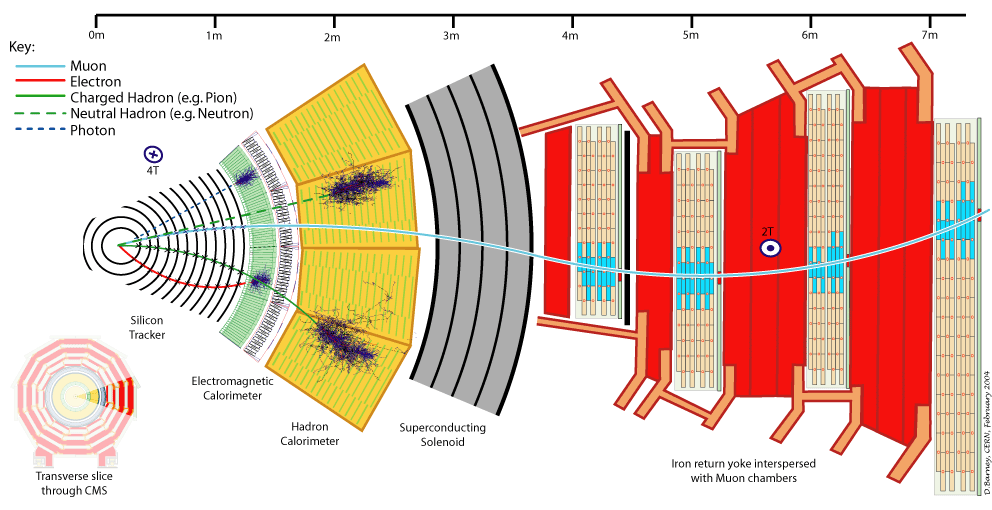
\includegraphics[width=\textwidth]{figures/CMSSlice.png}
  \caption{Transverse slice of the CMS detector \cite{Davis:2205172}, illustrating the basic structure of CMS and the shapes of the tracks and energy deposits formed by the five general categories of particles directly detected by CMS by one or more of its subsystems.}
  \label{cms:interactive}
\end{figure}
It also shows the detector signatures of the general categories of particles directly detected by CMS:
\begin{itemize}
  \item electrons
  \item photons
  \item charged hadrons
  \item neutral hadrons
  \item muons
\end{itemize}
The charged particles -- electrons, muons, and charged hadrons -- are detected as they form curved, helical tracks in the silicon tracker (and in the case of muons, in the muon system as well).
Electrons, charged hadrons, and the neutral particles -- photons and neutral hadrons -- leave energy deposits in the electromagnetic and hadronic calorimeters.

\subsection{Coordinate System}
The origin of the coordinate system used by CMS is the nominal \pp collision point.
The $y$-axis points upwards, the $x$-axis points radially inwards towards the center of the LHC, approximately south, and thus the $z$-axis points approximately west.
The azimuthal angle $\phi$ is measured from the $x$-axis and the radial coordinate in the $xy$-plane is denoted $r$.
The polar angle measured from the $z$-axis is denoted $\theta$.
However, a more conventional coordinate used in hadron collider physics is the pseudorapidity $\eta$, defined as
\begin{equation}
  \eta = -\ln\tan\left(\frac{\theta}{2}\right)
  \label{eq:eta}
\end{equation}
For a particle of three-momentum $\vc{p}$ with $z$-component $p_z$, pseudorapidity can be written
\begin{equation}
  \eta = \frac12\ln\left(\frac{|\vc{p}|+p_z}{|\vc{p}|-p_z}\right)
  \label{eq:eta_p}
\end{equation}
This form elucidates its relationship to rapidity,
\begin{equation}
  y = \frac12\ln\left(\frac{E+p_z}{E-p_z}\right),
  \label{eq:rap}
\end{equation}
which is a quantity Lorentz invariant under boosts in the $z$-direction.
The pseudorapidity has the advantage that it converges to rapidity in the high-energy, low-mass limit (as $|\vc{p}|\to E$), but is only dependent on the polar angle $\theta$ and not on the energy of the particle.
\Fig~\ref{cms:quadrant} is a schematic diagram of one quadrant of CMS, showing the placement of the components of CMS within the coordinate system.
\begin{figure}[htpb]
  \centering
  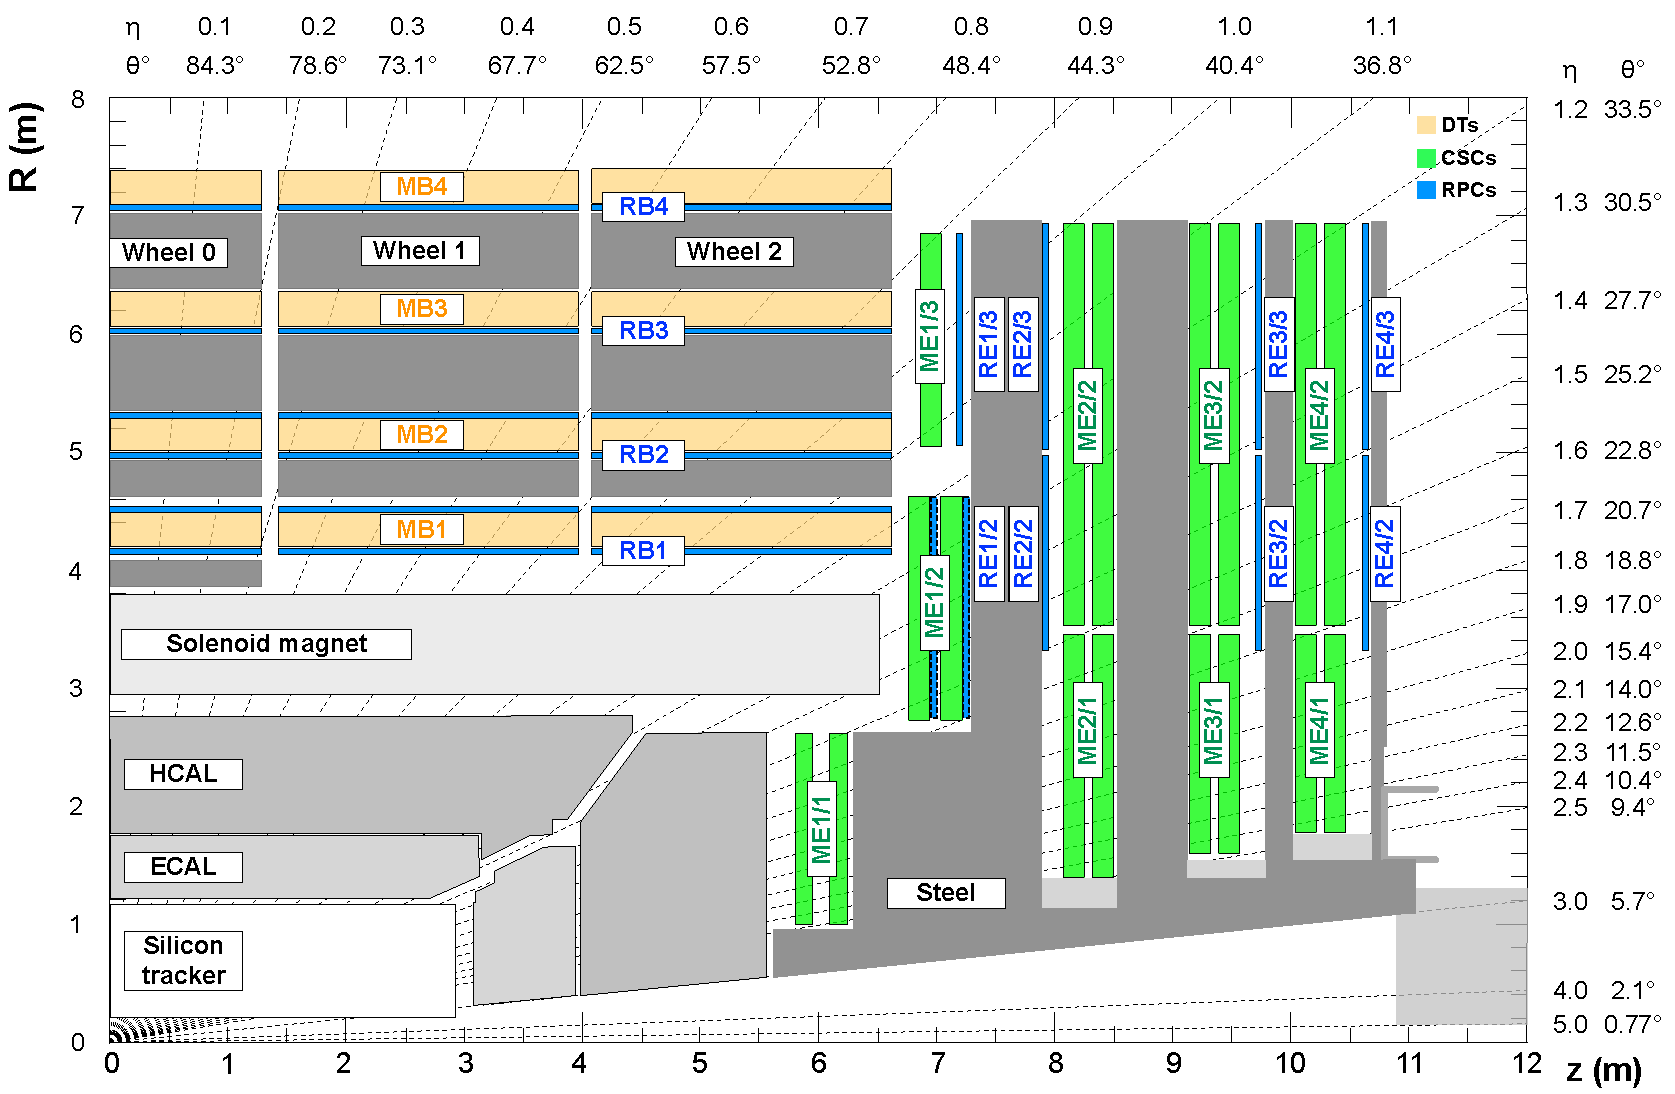
\includegraphics[width=\textwidth]{figures/CMSGeometry.pdf}
  \caption{Schematic diagram of one quadrant of CMS in $r$-$z$ \cite{Sirunyan:2018fpa}, illustrating the position of all the subsystems with respect to the coordinate system, in both the barrel and the endcap.}
  \label{cms:quadrant}
\end{figure}

The diagram illustrates that $\eta = 0$ points upwards, while $\eta \to \infty$ points along the $z$-axis.
For this reason the ``forward'' regions close to the beamline (which are also less instrumented) are referred to as ``high $\eta$.''
The diagram also illustrates two distinct loci within the CMS detector: the barrel, which covers approximately (depending on subsystem) the region $|\eta| < 1.2$, and the endcap, which covers approximately (depending on subsystem) the region $1.2 < |\eta| < 3$.

\subsection{Silicon Tracker}
The inner tracking system of CMS must provide precise measurements of charged particle trajectories and reconstructions of secondary vertices of (on average) a thousand particles every 25\unit{ns} bunch crossing, exposed to the full flux of the radiation of the LHC.
These requirements on precision, speed, and radiation hardness inform a choice of silicon detector technology.
The ionization produced by an energetic charged particle passing through induces produced electron-hole pairs, which are measured as current in the presence of an applied voltage.

The CMS tracker consists of two silicon detector technologies: pixels and strips.
The innermost component of the tracker, closest to the collision point, is the pixel detector, consisting of three barrel layers and two endcap disks on each side of the barrel.
The silicon pixel sensors are $n$-on-$n$ devices, measuring $100 \times 150 \mum^2$, giving a spatial resolution of 15--20\mum and a transverse momentum ($\pT$) resolution of 1\% for 100\GeV particles.
Just outside the pixel detector is the strip detector, consisting of ten barrel layers and twelve endcap disks on each side of the barrel.
The silicon strip sensors are $p$-on-$n$ type microstrip sensors, manufactured on 6\unit{in} wafers \cite{Chatrchyan:2008zzk, CERN-LHCC-98-006, HARTMANN201225}.


\subsection{Electromagnetic Calorimeter}
The electromagnetic calorimeter (ECAL) was designed to achieve the excellent energy resolution critical for observing the decay of the SM Higgs to two photons: $H \to \gamma\gamma$.
The ECAL is a homogeneous calorimeter consisting of lead tungstate (PbWO$_4$) crystals, a material chosen for its high density and short radiation length.
Scintillation is the operating principle of the ECAL.
Electrons or photons passing through the detector material result in a cascade of electromagnetic interactions, producing a shower of particles culminating in a release of energy proportional to the energy of the incident particle.
The corresponding photons are then measured by photodetectors installed on each crystal \cite{Chatrchyan:2008zzk, CERN-LHCC-97-033, Fabjan:692252}.

\subsection{Hadronic Calorimeter}
The hadronic calorimeter (HCAL) is a sampling calorimeter, meaning it consists of repeating, alternating layers of an absorber, which degrades the energy of an incident particle, and an active medium, which provides a detectable signal.
This is in contrast to a homogenous calorimeter, like the ECAL, in which a single type of material performs both functions.

The HCAL consists of four parts: the barrel and endcap HCAL (HB and HE), the outer HCAL (HO), and the forward HCAL (HF).
In the HB and HE, the absorber material consists of thick tiles of brass, and the active medium consists of thinner tiles of scintillating plastic with wavelength-shifting readout fibers.
Brass is a dense material with many nuclei to interact strongly with incident hadron showers.
It is also non-magnetic, a necessary property of the absorber for the HB and HE which lie within the solenoid and experience its full 4\unit{T} magnetic field.

As the HB and HE lie within the solenoid and hence are only about 6 interaction lengths thick, the first layer of the muon system is instrumented with scintillator tiles, treating the solenoid as an additional absorber.
This ``tail catcher'' is known as the outer calorimeter, or HO.

The HF is located 11\unit{m} from the interaction point, in the pseudorapidity range of approximately $3.0 < |\eta| < 5.0$.
This forward region experiences very high levels of LHC radiation and thus is constructed out of radiation-hard materials: steel for the absorber and quartz fiber for the active material, which detects the Cerenkov radiation produced by energetic jets \cite{Chatrchyan:2008zzk, CERN-LHCC-97-031, Penzo2009}.

\subsection{Muon System}
\subsubsection{Drift Tubes}
\subsubsection{Resistive Plate Chambers}
\subsubsection{Cathode Strip Chambers}

\subsection{Trigger and Data Acquisition Systems}
